\documentclass{article}

\usepackage{../preamble}
\standalonetrue

\title{MATH 316 Lecture 6}
\author{Ashtan Mistal}
\date{May 19 2021}

\begin{document}

\ifstandalone
\maketitle
\fi

\graphicspath{{./Lecture06/}}

\section{Recap of Frobenius Series Solutions}

Assume $x_0$ is a singular point of the ODE of the form:

$$P(x) y'' + Q(x) y' + R(x) y = 0$$

If $x_0$ is a regular singular point,

$$\lim_{x \to x_0} \frac{Q(x)}{P(x)} x = p_0$$

and

$$\lim_{x \to x_0} \frac{R(x)}{P(x)} x^2 = q_0$$

The characteristic equation is:

$$r(r-1) + p_0 r + q_0 = 0 \longrightarrow \text{2 roots: } r_1, r_2$$

For $r_1$, we get $y_1(x) = |x|^{r_1} \left( 1 + \sum_{n= 1}^{\infty} a_n x^n \right) = \sum_{n = 0}^\infty a_n x^{n + r_1}$

$a_n$ is found from a recursion by substitution into the ODE. $a_0$ is arbitrary. 

\hfill

1) If $r_1 - r_2 \neq 0$ and $r_1 - r_2 \neq N$ (N is an integer), then:

$$y_2 = |x|^{r_2} \left(1 + \sum_{n = 1}^\infty a_n x^n \right) = \sum_{n = 0}^\infty a_n x^{n + r_2}$$

2) If $r_1 = r_2$:

$$y_2(c) = y_1 (x) \ln(x) + |x| ^{r_1} \sum_{n = 1}^\infty C_n x^n = y_x(x) \ln(x) + \sum_{n = 1}^\infty C_n x^{n + r_1}$$

Note that $x > 0$. 

\hfill

Where $c_n = a_n ' = \left. \frac{d a_n}{dr} \right|_{r = r_1}$


Note 1: What happens of $r_1$ and $r_2$ are complex?

If they are, the form of $y_2$ in 1) (that we discussed), and $y_1$ are still valid; we just need to convert complex valued to real valued solutions. Needs lots of algebra. 

Note 2: A summary of these solutions is given in the formula sheet for the exam. 

Note 3: The general solution is in the following format:

$$y(x) = C_1 y_1(x) + C_2 y_2(x)$$

\hfill

\section{PDEs}

Continued from last class's notes. 

\subsubsection{Heat equation / diffusion equation}

$$\frac{\partial u}{\partial t} = k \frac{\partial^2 u}{\partial x^2} + k \left(\frac{\partial^2 u}{\partial y^2} + \frac{\partial^2 u}{\partial z^2} \right)$$

Applications: heat flows, diffusion of chemical substances

\subsubsection{Wave equation}

$$\frac{\partial^2 u}{\partial t^2} = C^2 \frac{\partial^2 u}{\partial x^2} + C^2 \left(\frac{\partial^2 u}{\partial y^2} + \frac{\partial^2 u}{\partial z^2}\right)$$

Applications: Vibrations, acoustics, solid mechanics

\subsubsection{Laplace's equation}

$$0 = \frac{\partial^2 u}{\partial z^2} + \frac{\partial^2 u}{\partial y^2}$$

Applications: Heat / wave equations in which there is a steady-state solution (eg potential flow, porous media flow)

\subsection{Classification of PDEs}

\hfill

ODEs: $f(x,u(x), u'(x)) = 0$. e.g. $u' = e^u$

\hfill

PDEs: $\underbrace{a(x,y) u_x + b(x,y) u_y = c(x,y) u}_{\text{First order, linear PDE}}$

\hfill

The solution to a PDE would look like a 2d surface: 

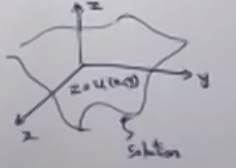
\includegraphics[width = 0.7 \textwidth]{image1.png}

Another example of a surface from WolframAlpha:

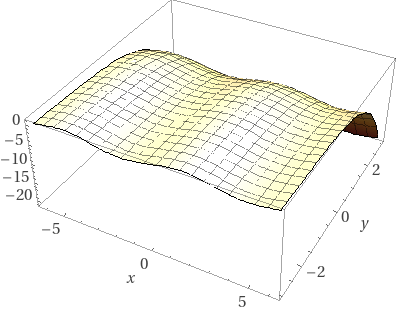
\includegraphics[width = 0.7 \textwidth]{image6.png}

\hfill

This course primarily focuses on second order linear PDEs. 
\begin{equation}
    A u_{xx} + 2 B u_{xy} + C u_{yy} + D u_x + E u_y + Fu = G
\end{equation}

$A,B,C,D,E,F,G$ can either be constants or functions of $(x,y)$.

The examples that we saw (heat equation, wave eq, etc) are all examples of the above (1). 

\hfill


If $G = 0$, the PDE is homogeneous. Else, it is non-homogeneous. 

To classify PDEs we use the analogy with corresponding quadratic surfaces:

$$AX^2 + BXY + CY^2 + DX + EY = K$$

To classify, we use the discriminant:

$$\Delta = B^2 - 4AC$$

It tells us either ellipse ($\Delta < 0$), hyperbola ($\Delta > 0$), or a parabola ($\Delta = 0$)

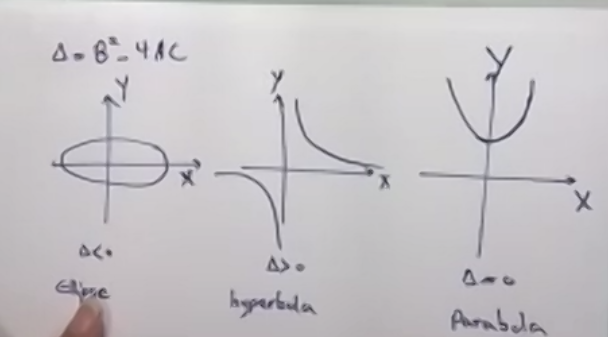
\includegraphics[width = 0.9 \textwidth]{image2.png}

$$\begin{matrix} 
\Delta & \text{Type} & \text{PDE} & \text{Note} \\ 
\Delta = 0 & \text{parabolic} & u_t = u_{xx} & \text{Heat eq} \\ 
\Delta < 0 & \text{elliptic} & u_{xx} + u_{yy} = 0 & \text{Laplace eq} \\
\Delta < 0 & \text{elliptic} & u_{xx} + u_{yy} = G & \text{Poisson's eq} \\
\Delta > 0 & \text{Hyperbolic} & u_{tt} = c^2 u_{xx} & \text{Wave eq}
\end{matrix}$$

\hfill

\subsection{Heat / Diffusion Equation}

Consider a rod of length $\Delta x$:

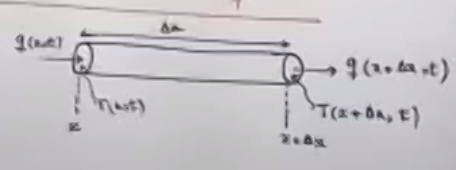
\includegraphics[width = 0.9 \textwidth]{image3.png}

\hfill

(The equations that are a bit blurry are the following, left to right and top to bottom: $q(x,t)$, $\Delta x$, $q(x + \Delta x, t)$, $T(x,t)$, $T(x + \Delta x, t)$, $x$, $x + \Delta x$)
\begin{itemize}
    \item $T(x,t)$: Temperature at $(x,t)$
    \item $q(x,t)$: The heat flux (heat energy per unit area)
    \item $C$: The specific heat capacity
    \item $\rho$: density of material
    \item $A$: The cross sectional area
\end{itemize}


Energy conservation: The increase in the thermal energy of the bar is equal to the (influx - outflux) of heat.  (Physical description, not mathematical description). 

Use variables: $C (T(x,t + \Delta t) - T(x,t)) \rho \Delta x A = (q (x,t) - q(x + \Delta x, t)) A \Delta t$

Divide by $\Delta t \cdot \Delta x$: 

$$\rho C \frac{T(x,t + \Delta t) - T(x,t)}{\Delta t} = \frac{q(x,t) - q(x,t + \Delta t)}{\Delta x}$$

As $\Delta t \to 0$ and $\Delta x \to 0$:

$$\rho C \frac{\partial T}{\partial t} = - \frac{\partial q}{\partial x}$$

The energy conservation equation is hence:

\begin{equation}
\label{energy conservation equation}
    \frac{\partial q}{\partial x} + \rho C \frac{\partial T}{\partial t} = 0
\end{equation}

In order to reduce the number of dependent variables, we need a constitutive equation between $q$ and $T$. Can we relate the heat flux to the temperature?

Yes. The heat transfer through conduction is formulated as:
\begin{equation}
\label{Fourier's Law}
\tag{Fourier's Law}
    q = -k \frac{\partial T}{\partial x}
\end{equation}

where $k$ is the thermal conductivity of the material. What does this tell us?

- Heat flux will flow from high temperature to low temperature. 

We can substitute \ref{Fourier's Law} in the energy conservation equation:

$$-k \frac{\partial^2 T}{\partial x^2} + \rho c \frac{\partial T}{\partial t} = 0$$

$$\hookrightarrow \frac{\partial T}{\partial t} = \alpha^2 \frac{\partial T}{\partial x^2}$$

Where $\alpha^2 = \frac{k}{\rho c}$ (diffusion coefficient). 

\subsection{Solving diffusion equations using separation of variables}

The initial boundary value problems, $u_t = \alpha^2 u_{xx}$, needs one initial condition (IC) and two boundary conditions (BC). 

Initial condition: $u(x,t = 0) = f(x)$ on the domain $0 < x < L$

\subsubsection{Boundary conditions}

(1) Dirichlet boundary conditions $u(0,t) = 0 = u(L,t)$ (i.e. same temperature on either side of the rod). Temperature is fixed: (see screenshot below). 

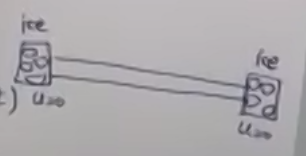
\includegraphics[width = 0.5 \textwidth]{image4.png}

(2) Neumann boundary conditions: $u_x (0,t) = 0 = u_x (L,t)$. i.e. insulation on either side of a rod. Temperature won't change with respect to $x$. 

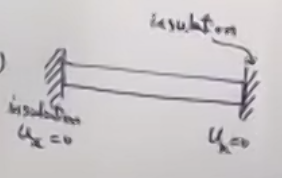
\includegraphics[width = 0.5 \textwidth]{image5.png}

(3): Mixed boundary conditions. $u(0,t) = 0$ and $u_x (L,t) = 0$

\subsubsection{Example 1}
\begin{center}
    $u_t = \alpha^2 u_{xx}$, $0 < x < L$, $t > 0$
\end{center}


Boundary conditions:

$$\begin{matrix} u(0,t) = 0 \\ u(L,t) = 0 \end{matrix}$$

Initial conditions: $$u(x,0) = f(x)$$

To solve, we use the method of separation of variables. We will do this next class. 

\end{document}
